\documentclass[12pt]{article}
\usepackage{graphics, graphicx, tabularx, fancyhdr, amsmath, lastpage, indentfirst, lscape, algorithm, algorithmic, siunitx}
\usepackage[margin=1in]{geometry}
\usepackage[super, sort&compress, comma]{natbib}

% define variable for OSX vs. Windows path to Dropbox folder
% \def \dropboxpath {D:/Dropbox/} % for windows
\def \dropboxpath {/Users/rmuraglia/Dropbox/} % for osx

% define spacing for paragraph indent and space between paragraphs
% \setlength{\parindent}{4ex}
% \setlength{\parskip}{0ex}

% set custom header and footers
\pagestyle{fancy}
\fancyhf{} % remove current presets
%\renewcommand{\headrulewidth}{0pt} %uncomment to remove header line separator
\fancyhf[EOHL]{Job test - write up} % evens, odds, header, left
\fancyhf[EOHR]{Ryan Muraglia} % events, odds, header, right
\fancyhf[EOFC]{\thepage / \pageref{LastPage}} % evens, odds, footer, center
\setlength{\headheight}{15pt} % might throw a warning about minimum height: adjust this to fix

% create custom method for delimiting days: draws a short centered line and aligns the new date to the right
\newcommand{\newday}[1]{
\centerline{ \rule{3in}{0.4pt}} 

\hfill \emph{#1} \\
}

% redefine list structures to be more compact
\let\oldenumerate\enumerate
\renewcommand{\enumerate}{
  \oldenumerate
  \setlength{\itemsep}{1pt}
  \setlength{\parskip}{0pt}
  \setlength{\parsep}{0pt}
  % \vspace{-2ex}
}

% macro for red text for annotating drafts
\usepackage{color}
\newcommand{\redtext}[1]{
  \textcolor{red}{#1}
}

\begin{document}

\section{Model Comparison} % (fold)
\label{sec:model_comparison}

\subsection{LASSO} % (fold)
\label{sub:lasso}

The LASSO is a variant of linear regression which uses an $\ell_1$ penalty term to enforce shrinkage and sparsity in the coefficients. 
The objective function, which we minimize with respect to $\beta$ is:
\begin{equation}
  f_{LASSO}(\beta) = \sum (y - \beta X)^2 + \alpha \sum_{i=1}^p |\beta_i|
\end{equation}
where $\alpha$ controls the regularization strength, with higher values of $\alpha$ leading to more sparsity.

Some pros of the LASSO are:
\begin{enumerate}
  \item Feature selection: due to the $\ell_1$ penalty term, regression coefficients can be zeroed out (as opposed to in Ridge regression, or Tikhonov regularization with uses an $\ell_2$ penalty term, where coefficients are shrunk towards zero, but rarely, if ever zeroed out).
  \item High model interpretability: with fewer features with non-zero coefficients, we only need to focus on the role of a potentially small subset of covariates, allowing us to gain a stronger intuition of their impact.
  \item Protection from overfitting: like other regularized regression techniques, the main benefit of the LASSO is to prevent overfitting by simplifying the regression model. In other words, the LASSO tends to be robust to the training data and learns similar models.
\end{enumerate}

Some cons of the LASSO are:
\begin{enumerate}
  \item $\alpha$ selection: we need to choose a value for the shrinkage parameter. We can overcome this drawback by using a cross validation scheme to choose a good value.
  \item Non linear relationships: as with all linear regression methods, LASSO cannot accurately learn non-linear relationships without the introduction of modified features, like polynomial expansions or log transforms.
  \item Non-sparse situations: in the event that many of the features are important, enforcing sparsity can lead to a reduction in the prediction accuracy, due to the removal of potentially informative covariates.
\end{enumerate}

% subsection lasso (end)

\subsection{Decision Tree Regression} % (fold)
\label{sub:decision_tree_regression}

Decision trees are a class of modeling algorithms based on simple graphs.
Although more commonly thought of for their use in classification, tree-based methods can also be used for regression. 
Decision trees work by recursively partitioning the feature space based on simple rules to bin observations into groups.
To predict the value for a new, unseen observation, one simply needs to traverse the tree, following the rule at each node until it reaches a leaf of the tree (a bin).
Once binned, a value can be predicted based on the training examples in that bin (e.g. the mean of the variable of interest for those samples).

Some pros of decision tree regression are:
\begin{enumerate}
  \item Non-parametric learning: unlike linear regression, decision trees have no underlying parametric form, allowing them to learn non-linear relationships effectively.
  \item Intuitive to understand: the decision tree can be visualized easily, the most important decision rules are close to the root of the tree, and the decision rules themselves tend to be very simple (e.g. ``is the k-th feature greater than 50? Yes or No.''), so tracing how samples are being binned is easy.
  \item Minimal data preparation: trees operate on simple univariate comparisons, so standardization of variables, or special treatment for categorical variables is not necessary.
\end{enumerate}

Some cons of decision tree regression are:
\begin{enumerate}
  \item Risk of overfitting: if the depth of the tree is not controlled, decision trees will tend to overfit the training data, learning overly specific decision rules. This can be tempered by pruning the tree, or learning an optimal maximum depth based on cross validation.
  \item Complex relationships are difficult to learn: basic trees only learn univariate decision rules. If a critical predictor depends on the relationship between two or more variables, a decision tree will have a hard time capturing that interaction.
  \item Unstable tree generation: decision trees are relatively sensitive to the training data, and can learn different tree structures with a modest change in training data. This instability can be mitigated by ensemble based methods like random forests, which generate a number of decision trees based on random subsamples of the training data, which then aggregate their predictions together.
\end{enumerate}

% subsection decision_tree_regression (end)

% section model_comparison (end)

\section{Design Choices} % (fold)
\label{sec:design_choices}

Although not necessary for the work assignment, I thought it would be useful to discuss some key design choices and assumptions I made when preparing the data to give more information for your evaluation.

\subsection{Treatment of X15: ``Date loan was issued''} % (fold)
\label{sub:treatment_of_x15_}
This variable was encoded differently in the training and test sets. In the training set, it was encoded as ``Mon-XX'' where ``XX'' represented a year, and ``Mon'' a month. In the test set, X15 was encoded as ``XX-Mon'', where ``XX'' was always equal to 15. I worked under the assumption that the 15 in the test set referred to the year 2015.
% subsection treatment_of_x15_ (end)

\subsection{Treatment of X9: ``Loan subgrade''} % (fold)
\label{sub:treatment_of_x9_}
Because this variable appeared to be strongly predictive of income rate (see figure 1), I chose to impute the values using a more sophisticated scheme than using the mode, or using samples drawn randomly in proportions equal to those observed in the training set. 
I calculated the group median X1 for each category in X9, then assigned missing X9 values to the nearest group median.
Additionally, although this is a categorical variable, there is an implied ordering, and as such, I treated it as an ordinal variable, instead of an unordered categorical.

\begin{figure}
  \centering
  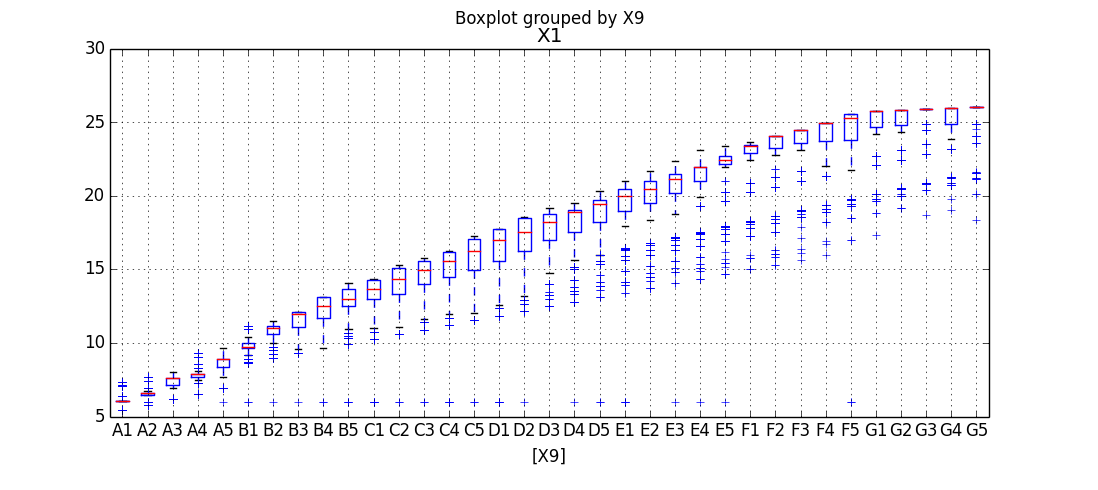
\includegraphics[scale=0.5]{X1_X9.png}
  \caption{Interest rate vs. Loan subgrade in the training set}
  \label{fig:figure1}
\end{figure}
% subsection treatment_of_x9_ (end)

\subsection{X4, X5 and X6} % (fold)
\label{sub:x4_x5_and_x6}
These variables, representing various aspects of the loan amount (requested, funded and investor-funded portion, respectively), appeared to have some degree of collinearity. 
I noted that X4 $\geq$ X5 $\geq$ X6, and as such we could encode X5 and X6 as boolean variables denoting their equality relationship to X4 and X5, respectively, which would provide an alternate perspective on the relationship between these variables.
Ultimately, I chose to keep X4, X5 and X6 as is, due to their minor importance in both models.
% subsection x4_x5_and_x6 (end)

\subsection{Redundant features} % (fold)
\label{sub:redundant_features}
In this dataset there were two sets of clearly redundant features. 
X8 and X9 represented loan grade and loan subgrade, respectively. As the subgrade provided more resolution for prediction, I chose to keep that feature.
X19 and X20 both represented spatial information, but because X19 was on a zip code level resolution, it generated over 300 categories, which was overkill, so I chose to drop that feature.
% subsection redundant_features (end)

% section design_choices (end)

\end{document}


